% Generated by pipeline/paper/scripts/make_result_figures.py. Do not edit by hand.
% Relative error of fitted stock on every sampled genome. The band is the 0.10 flag. Every genome is outside it.
% Shared figure style. Input once; a second input is a no-op.
\ifdefined\actsplotsready
\else
  \def\actsplotsready{1}
  \colorlet{actsteal}{teal!72!black}
  \colorlet{actstealfaint}{teal!16}
  \colorlet{actsorange}{orange!88!black}
  \colorlet{actsink}{black!80}
  \colorlet{actsghost}{black!45}
  \colorlet{actsfail}{red!62!black}
  \colorlet{actsrule}{black!50}
  \usetikzlibrary{intersections}
  \usepgfplotslibrary{fillbetween,groupplots}
  \pgfplotsset{
    acts/.style={
      font=\scriptsize\sffamily,
      tick label style={font=\scriptsize\sffamily},
      label style={font=\scriptsize\sffamily},
      legend style={
        font=\scriptsize\sffamily,
        draw=none,
        fill=none,
        cells={anchor=west},
        inner sep=1pt,
        column sep=6pt
      },
      legend cell align=left,
      scale only axis,
      clip=false,
      axis line style={actsrule},
      tick style={actsrule},
      tick align=outside,
      axis lines=left,
      xmajorgrids=true,
      major grid style={black!7},
      ymajorgrids=false,
      every node/.append style={font=\scriptsize\sffamily, inner sep=1.5pt},
      every axis plot/.append style={line join=round, line cap=round},
    },
  }
  \tikzset{
    actlab/.style={
      font=\scriptsize\sffamily,
      fill=white,
      fill opacity=0.92,
      text opacity=1,
      inner sep=1.35pt,
      outer sep=0.5pt,
    },
  }
\fi

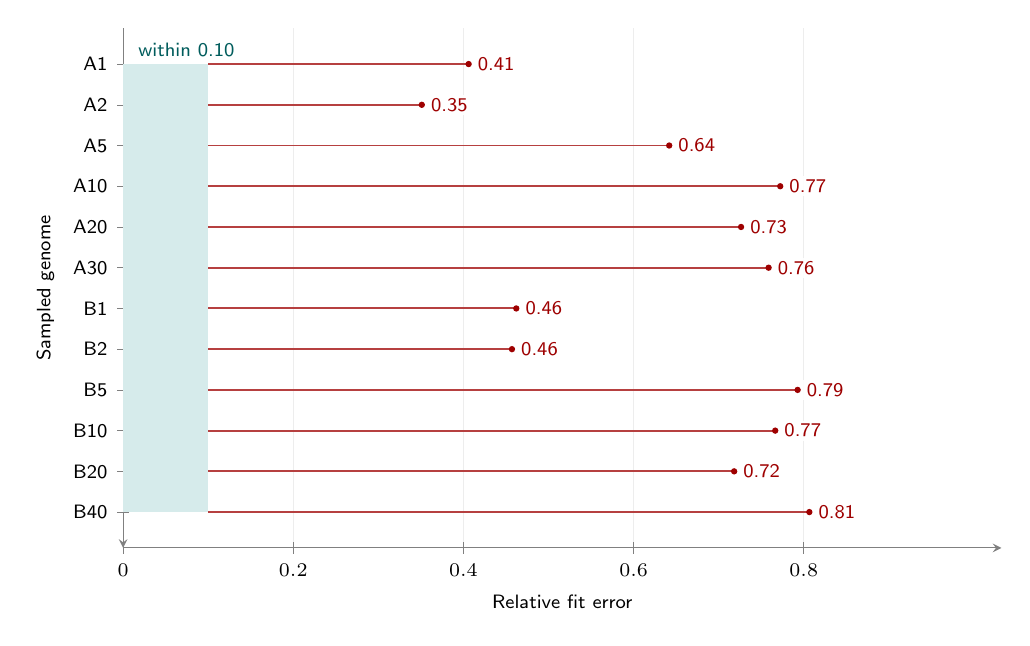
\begin{tikzpicture}
\begin{axis}[
  acts,
  width=0.92\columnwidth,
  height=6.6cm,
  xmin=0, xmax=1.03241,
  xtick={0,0.2,0.4,0.6,0.8},
  xlabel={Relative fit error},
  symbolic y coords={r0,r1,r2,r3,r4,r5,r6,r7,r8,r9,r10,r11},
  ytick={r0,r1,r2,r3,r4,r5,r6,r7,r8,r9,r10,r11},
  y dir=reverse,
  yticklabels={{A1},{A2},{A5},{A10},{A20},{A30},{B1},{B2},{B5},{B10},{B20},{B40}},
  enlarge y limits=0.08,
  ylabel={Sampled genome},
]
\addplot[draw=none, forget plot] coordinates {(0,r0) (0,r1) (0,r2) (0,r3) (0,r4) (0,r5) (0,r6) (0,r7) (0,r8) (0,r9) (0,r10) (0,r11)};
% source: locked flag |predicted-measured|/measured > 0.10
\fill[actstealfaint] (axis cs:0,r0) rectangle (axis cs:0.1,r11);
\node[actlab, anchor=south west, text=actsteal, yshift=1pt] at (axis cs:0.012,r0) {within 0.10};
\draw[actsfail!75, line width=0.7pt] (axis cs:0.1,r0) -- (axis cs:0.40610034,r0);
\fill[actsfail] (axis cs:0.40610034,r0) circle[radius=1.15pt];
\node[actlab, anchor=west, text=actsfail, xshift=1.5pt] at (axis cs:0.40610034,r0) {0.41};
\draw[actsfail!75, line width=0.7pt] (axis cs:0.1,r1) -- (axis cs:0.35106536,r1);
\fill[actsfail] (axis cs:0.35106536,r1) circle[radius=1.15pt];
\node[actlab, anchor=west, text=actsfail, xshift=1.5pt] at (axis cs:0.35106536,r1) {0.35};
\draw[actsfail!75, line width=0.7pt] (axis cs:0.1,r2) -- (axis cs:0.64186398,r2);
\fill[actsfail] (axis cs:0.64186398,r2) circle[radius=1.15pt];
\node[actlab, anchor=west, text=actsfail, xshift=1.5pt] at (axis cs:0.64186398,r2) {0.64};
\draw[actsfail!75, line width=0.7pt] (axis cs:0.1,r3) -- (axis cs:0.77235522,r3);
\fill[actsfail] (axis cs:0.77235522,r3) circle[radius=1.15pt];
\node[actlab, anchor=west, text=actsfail, xshift=1.5pt] at (axis cs:0.77235522,r3) {0.77};
\draw[actsfail!75, line width=0.7pt] (axis cs:0.1,r4) -- (axis cs:0.72631143,r4);
\fill[actsfail] (axis cs:0.72631143,r4) circle[radius=1.15pt];
\node[actlab, anchor=west, text=actsfail, xshift=1.5pt] at (axis cs:0.72631143,r4) {0.73};
\draw[actsfail!75, line width=0.7pt] (axis cs:0.1,r5) -- (axis cs:0.75870519,r5);
\fill[actsfail] (axis cs:0.75870519,r5) circle[radius=1.15pt];
\node[actlab, anchor=west, text=actsfail, xshift=1.5pt] at (axis cs:0.75870519,r5) {0.76};
\draw[actsfail!75, line width=0.7pt] (axis cs:0.1,r6) -- (axis cs:0.46211569,r6);
\fill[actsfail] (axis cs:0.46211569,r6) circle[radius=1.15pt];
\node[actlab, anchor=west, text=actsfail, xshift=1.5pt] at (axis cs:0.46211569,r6) {0.46};
\draw[actsfail!75, line width=0.7pt] (axis cs:0.1,r7) -- (axis cs:0.45703673,r7);
\fill[actsfail] (axis cs:0.45703673,r7) circle[radius=1.15pt];
\node[actlab, anchor=west, text=actsfail, xshift=1.5pt] at (axis cs:0.45703673,r7) {0.46};
\draw[actsfail!75, line width=0.7pt] (axis cs:0.1,r8) -- (axis cs:0.79280132,r8);
\fill[actsfail] (axis cs:0.79280132,r8) circle[radius=1.15pt];
\node[actlab, anchor=west, text=actsfail, xshift=1.5pt] at (axis cs:0.79280132,r8) {0.79};
\draw[actsfail!75, line width=0.7pt] (axis cs:0.1,r9) -- (axis cs:0.76646645,r9);
\fill[actsfail] (axis cs:0.76646645,r9) circle[radius=1.15pt];
\node[actlab, anchor=west, text=actsfail, xshift=1.5pt] at (axis cs:0.76646645,r9) {0.77};
\draw[actsfail!75, line width=0.7pt] (axis cs:0.1,r10) -- (axis cs:0.71819596,r10);
\fill[actsfail] (axis cs:0.71819596,r10) circle[radius=1.15pt];
\node[actlab, anchor=west, text=actsfail, xshift=1.5pt] at (axis cs:0.71819596,r10) {0.72};
\draw[actsfail!75, line width=0.7pt] (axis cs:0.1,r11) -- (axis cs:0.80657293,r11);
\fill[actsfail] (axis cs:0.80657293,r11) circle[radius=1.15pt];
\node[actlab, anchor=west, text=actsfail, xshift=1.5pt] at (axis cs:0.80657293,r11) {0.81};
% source: savings_20261006/A_hmmsearch.json and B_hmmsearch.json stock_pred_rel_error
\end{axis}
\end{tikzpicture}
